\section{Background}

\subsection{RAG Architectures and LLMs}

Research on retrieval-augmented generation (RAG) architectures in language models (LLMs) has predominantly focused on enhancing LLMs' ability to generate contextually relevant and information-rich content by leveraging external knowledge bases. The initial exploration presented an innovative approach by combining the transformer architecture with a dynamic external memory. The authors highlighted the model's proficiency in contextual understanding and its applications across various domains such as chatbots and information retrieval systems. However, a notable limitation identified was the latency introduced due to the retrieval process, which impacts the real-time response capabilities of the models \parencite{lewis2020retrieval}. \\

\begin{figure}[H]
\centering
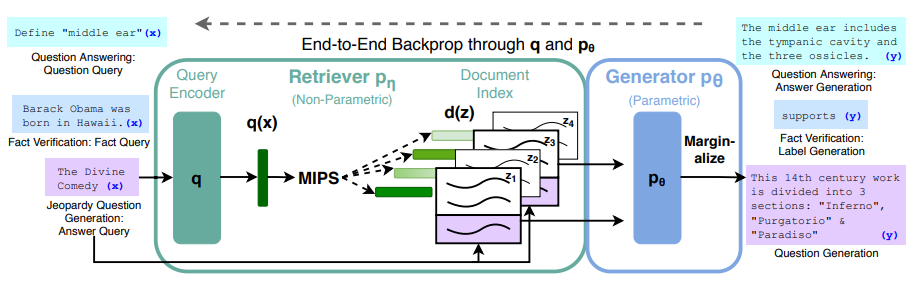
\includegraphics[width=0.8\textwidth]{Ref. 1.png}
\caption{Overview of a Retrieval-Augmented Generation Model \parencite{lewis2020retrieval}}
\end{figure}

Figure 1 gives an overview of the working mechanism of the RAG model. RAG models find and use relevant text (z) to help generate answers (y) based on a query (x). They consist of a retriever, which finds related content, and a generator that creates responses based on this content and the query context. \\

Building on this, researchers expanded the RAG architecture's application to more complex tasks including summarization and question answering. Johnson and colleagues refined the retrieval process to improve efficiency and introduced a multi-vector retrieval system that reduces the time overhead. Despite these improvements, the paper noted a persistent challenge with the scalability of the model when interfaced with significantly large data sets, which often led to decreased precision in retrieval outcomes \parencite{gao2023retrieval}.

\begin{figure}[H]
\centering
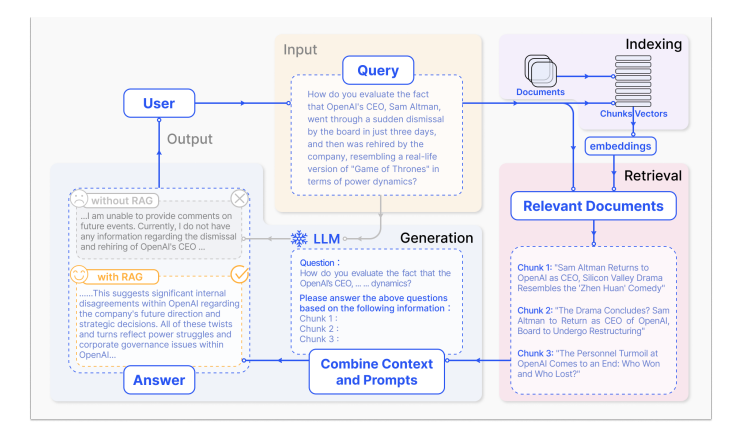
\includegraphics[width=0.8\textwidth]{Ref. 2.png}
\caption{A representative instance of the RAG process applied to QA \parencite{gao2023retrieval}}
\end{figure}

Figure 2 illustrates a RAG model for answering questions: It first creates a searchable index of document parts, then finds the most relevant parts to a question, and finally uses those parts to generate an answer.

\subsection{Information Retrieval using LLMs}

Further study delves into integrating information retrieval (IR) techniques directly with LLMs, without the intermediary of traditional RAG components. This integration aims to streamline the retrieval process by embedding IR functionalities within the LLM framework itself. The authors demonstrated that this direct integration allows for faster retrieval times and enhances the relevance of the information retrieved, contributing to more accurate and context-aware responses from LLMs. However, the study also highlighted a limitation in terms of adaptability, where the LLM struggled to dynamically adjust to new or evolving data types without manual interventions \parencite{ai2023information}.

\subsection{Temporal Awareness in LLMs}

Advancements in temporal awareness within LLMs have been marked by a series of studies focused on embedding a sense of 'time' or 'history' into the models. 
Further research introduced a framework that allows LLMs to maintain stateful interactions over time, which significantly improves their utility in continuous interaction environments like digital assistants and monitoring systems. However, the authors noted that maintaining accuracy with increasing temporal distance remains challenging \parencite{chen2023temporal}. \\

Other researchers built on this by introducing methods to integrate these temporal frameworks with existing LLM architectures more efficiently. Innovations such as the use of a temporal attention mechanism were highlighted, which enables the LLM to focus on relevant parts of a stored conversation or document based on the time cues. Yet, these methods still face challenges in terms of computational efficiency and the complexity of training with temporal data. \parencite{zhang2024event,mann2020language}. \\

Further exploration introduced more refined temporal encoding techniques, aiming to reduce the resource demands and improve the model's ability to generalize across different temporal contexts. Each step forward in the research demonstrated a progressive enhancement in handling temporal data, but also underscored the need for more robust training datasets that are temporally varied to train these models effectively \parencite{kynoch2023recallm,dhingra2022time}.

\subsection{Temporal Awareness in IR}

The exploration of temporal awareness in information retrieval (IR) systems has significantly advanced with research focused on integrating temporal dimensions into IR frameworks. Recent research introduced a novel approach for enhancing traditional IR systems with temporal tagging capabilities that allow for the sorting and retrieval of information based on time-specific criteria. This model showed promising results in improving the relevance of retrieved documents for time-sensitive queries, though it struggled with the accuracy of temporal tagging in noisy data environments \parencite{moulahi2016time}. \\

"Building on this, another study extended the concept by incorporating a machine learning model that predicts the temporal relevance of documents based on their content and metadata. This system was able to dynamically adjust its retrieval strategies based on the temporal intent of the queries. However, the model required extensive training data to effectively understand and categorize temporal expressions, which limited its immediate applicability in smaller or less structured datasets \parencite{whiting2016temporal}. \\

Other researchers implemented an advanced algorithm that combines the features of the previous studies with a real-time updating mechanism to handle streaming data. Their system demonstrated the ability to update its index with new information while maintaining an accurate temporal context. Despite these advancements, the complexity of the algorithm led to challenges in deployment, particularly in resource-constrained environments \parencite{campos2014survey}.

\subsection{Temporal Awareness in QA Systems}

The integration of temporal awareness into QA systems has been markedly advanced through the development of the Time-Sensitive QA dataset \parencite{chen2021dataset}. This dataset is designed to challenge and benchmark QA systems on their ability to handle time-sensitive questions that require understanding and reasoning over temporal information. The dataset effectively highlights the shortcomings of current state-of-the-art QA systems, which typically achieve only about 46\% accuracy compared to human performance at 87\%, underscoring a significant gap in the ability to handle temporal reasoning. The authors suggest that the development of new models trained on this dataset could lead to significant improvements in automated systems' understanding of time-sensitive information.